\documentclass[tikz]{standalone}
\begin{document}
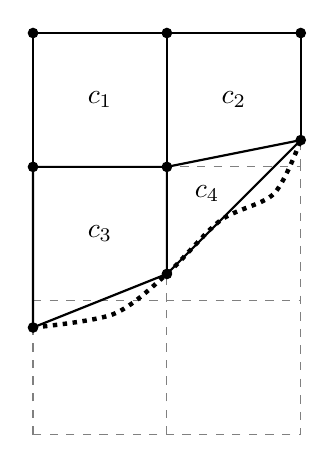
\begin{tikzpicture}[
  scale=0.17
]

\draw [dashed, gray] (0,0) rectangle (20, 20);
\draw [dashed, gray] (10,0) -- (10,20);
\draw [dashed, gray] (0,10) -- (20,10);
\draw [dashed, gray] (20,20) -- (20,30);

\draw [thick] (0,8) -- (0,20) -- (10,20) -- (10,12) -- (0,8);
\draw [thick] (10,20) -- (20,22) -- (10,12);
\draw [thick] (0,20) -- (0,30) -- (20,30) -- (20,22);
\draw [thick] (10,20) -- (10,30);
\draw [dotted, ultra thick] plot [smooth] coordinates {(0,8) (6, 9) (10,12) (14,16) (18,18) (20,22)};
\fill (0,30) circle [radius=0.4];
\fill (0,20) circle [radius=0.4];
\fill (10,20) circle [radius=0.4];
\fill (10,30) circle [radius=0.4];
\fill (20,30) circle [radius=0.4];
\fill (0,8) circle [radius=0.4];
\fill (10,12) circle [radius=0.4];
\fill (20,22) circle [radius=0.4];
\node at (5,25) {$c_1$};
\node at (15,25) {$c_2$};
\node at (5,15) {$c_3$};
\node at (13,18) {$c_4$};

\end{tikzpicture}
\end{document}
